
\documentclass[10pt]{beamer}

\usepackage{graphicx}
\usepackage{amsfonts}
\usepackage{amsmath}
\usepackage{amssymb}
\usepackage[dvipsnames]{xcolor}
\usepackage[skip=10pt plus1pt] {parskip}

%Information to be included in the title page:
\title{Analysis}
\author{UChicago Political Science Math Camp}
\institute{Ryan Gibbons \& Luke Cain}
\date{2025}

\begin{document}

\frame{\titlepage}


\begin{frame}{Analysis of Functions}
Very rarely do we just want to ``know" a function that we are working with. We might ask the following \textcolor{red}{(why?)}:
\vspace{.2cm}
\begin{itemize}
    \item \textit{What does a function do near some point?}
    \item \textit{What does a function do as some input reaches infinity?}
    \item \textit{What are the highest/lowest values a function might output?}
\end{itemize}
\vspace{.5cm}
Some of these are easy. Others are fun!

\end{frame}


\begin{frame}{What is a Limit?}
    Conversationally, the \textbf{limit} represents the value a function approaches given an input behavior:

    \[\lim_{x \to b} f(x)\]

    represents the value that $f(x)$ approaches as $x$ approaches $b$. 
    
\end{frame}


\begin{frame}{Some Limits Are Trivial}

Focusing on finite limits, we can evaluate:

\begin{itemize}
    \item \[\lim_{x \to 2} x^2\] \pause
    \item \[\lim_{x \to 0} e^x\] \pause
    \item \[\lim_{x \to a}\frac{a}{x}\]
\end{itemize}
\end{frame}

\begin{frame}{Others... Aren't}

Some limits allow us to analyze functions that don't return a numerical value:

\begin{itemize}
    \item \textit{Infinite inputs:}
    \[\lim_{x \to \infty} x^2\]
    \pause
    \item \textit{Infinite outputs:}
    \[\lim_{x \to 0}\frac{1}{x^2}\]
    \pause
    \item \textit{Hole discontinuities:}
    \[\lim_{x \to 1} \frac{x^2 - 1}{x - 1}\]
\end{itemize}
    
\end{frame}

\begin{frame}{Convergence \& Divergence}
    A function \textbf{converges} if it gets very close to a constant value. Formally, \\
\vspace{1cm}
    \begin{quote}
        A function has a limit $\lim_{x \to p} f(x) = L$ iff for all $\epsilon > 0$, there exists some $\delta > 0$ such that $0 < |x - p| < \delta \implies |f(x) - L| < \epsilon$.
    \end{quote}
    \vspace{.25cm}
    If there is no $a$ for which this definition holds, then the sequence \textbf{diverges}. \\

    \vspace{.5cm}

    \textcolor{NavyBlue}{What does this mean conversationally?}
\end{frame}

\begin{frame}
    \begin{center}
        
\includegraphics[width=5cm]{diverge.jpg}
    \end{center}
\end{frame}


\begin{frame}{Some More Examples}
    \[\lim_{x \to \infty} x^2\] \pause

    \[\lim_{x \to \infty} \sqrt{x}\]
\end{frame}


\begin{frame}{There's Always Cauchy}
If the limit itself is unknown, Cauchy Convergence provides an alternative definition:

\vspace{.5cm}

\begin{quote}
        A function $f$ converges iff for all $\epsilon > 0$, there exists some $\delta$ such that $m,n > \delta \implies |f(m) - f(n)| < \epsilon$.
    \end{quote}

\vspace{.5cm}
    \textcolor{NavyBlue}{If the difference in subsequent values approaches zero, then the sequence/function must approach some constant.}
\end{frame}

\begin{frame}{An Illustrative Example: Redistribution}
    Boix (2003): Democracy is, in essence, a redistributive activity.

    Suppose a state has \underline{fixed total wealth} of $1$. There is a poor class with wealth $w_L$, and an elite class with wealth $w_H$.
    
    If redistribution from the wealthy to the poor happens repeatedly \underline{and fairly}, what will ultimately happen with $w_L$ and $w_H$? 

    \pause
    \textcolor{gray}{Logically, what can this suggest about persistent inequality?}
\end{frame}

\begin{frame}{Existence of Limits}

Let $\lim_{x \to a +} f(x)$ represent the right-side limit of $f(x)$ at $a$, and let $\lim_{x \to a-} f(x)$ represent the left-side limit. \\


\vspace{1.5cm}

\begin{quote}
    $\lim_{x \to a} f(x)$ exists iff  $\lim_{x \to a +} f(x) = \lim_{x \to a-} f(x)$.
\end{quote}

\vspace{.5cm}
This tends to affect two types of functional features:

\begin{enumerate}
    \item Piecewise
    \item Asymmetric vertical asymptotes
\end{enumerate}

\end{frame}

\begin{frame}{End Behavior}
    We are often interested in the \textbf{``end behavior"} of a function; i.e. its composition approaching infinity:

    \[\text{End behavior of } f(x) \equiv \lim_{x \to \infty} f(x)\]

    This usually results in $\lim_{x\to\infty}f(x) \in \{-\infty, a \in \mathbb{R}, \infty\}$
\end{frame}

\begin{frame}{Continuity}
Fundamentally, \textbf{continuity} is thought of as meaning ``one continuous line." But, is a function really a line? \\

\vspace{.5cm}

If only we had a convergence definition for function \textit{outputs}... \pause

\vspace{1cm}

\begin{quote}
    A function is continuous at point $c$ if $\lim_{x \to c} f(x) = f(c)$.
\end{quote}
\end{frame}


\begin{frame}{Differentiability}
    A function is \textbf{differentiable} over $[a,b]$ if for every $c \in [a,b]$, there exists a rate of change $m \in \mathbb{R}$. \\
\vspace{.5cm}
    \textit{(We will enhance this definition later on using derivatives.)}
\end{frame}

\begin{frame}{A Cool Math Fact: Brownian Motion}
    \begin{center}
        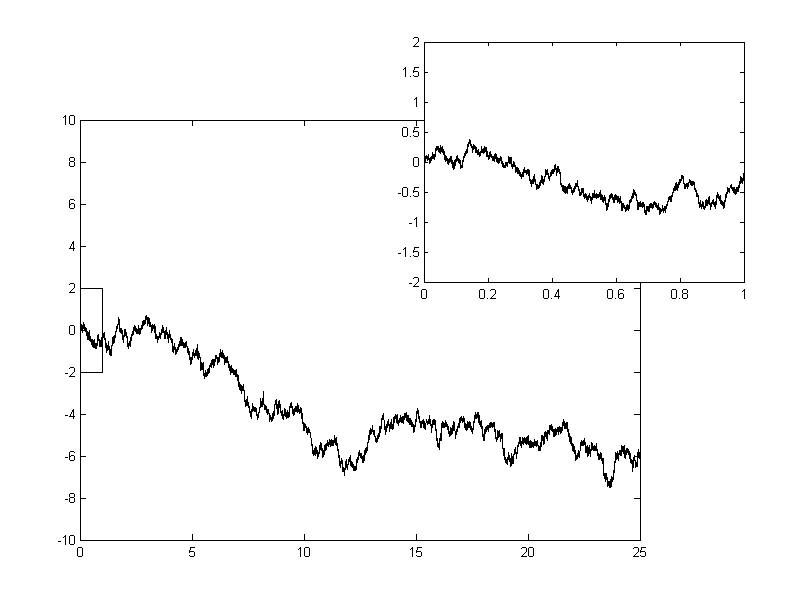
\includegraphics[width=10cm]{Wiener_process_zoom.png} \\
        \textit{\tiny{Wikimedia Commons}}
    \end{center}
\end{frame}


\begin{frame}{Extrema}
    The \textbf{\textcolor{red}{maxima} \textcolor{blue}{(minima)}} of a set is the element(s) of that set for which no other element is \textbf{\textcolor{red}{greater} \textcolor{blue}{(lesser)}}. \\

    \vspace{1cm}

    \textit{(This requires a \underline{well-ordering principle}, which is a property of $\mathbb{R}$ and its subsets.)}
\end{frame}


\begin{frame}{Maxima \& Minima}
    For most well-defined sets, finding maximal and minimal elements is straightforward \\

    \vspace{.3cm}

    We will see in Optimization that evaluating these for function co-domains is conceptually straightforward (even if technically challenging) \\

    \vspace{.3cm}

    We use the following notation in such cases (sub $max = min$):

    \[\max \{X\} = \text{Maximal element in set }X\]
    \[\max f(x) = \text{Maximal output of }f(x)\]
    \[\arg\max_x f(x) = \text{Value of $x$ which maximizes $f$}\]
\end{frame}


\begin{frame}{Can We Break This?}
    Let us define the following bijective function such that every real number is the output for a unique input:

    \[f: \mathbb{R}_+ \rightarrow \mathbb{R}_+ \quad \quad \quad f(x) = \frac{1}{x}\]

    We then evaluate:
    
    \[\max f(x)\]
    \pause
    \[\min f(x)\]
\end{frame}

\begin{frame}{We Broke It!}
    We can (and very frequently do) create well-defined sets which are \textbf{missing a well-defined extrema} \\

    \vspace{1cm}

    What aspect of our function's domain (along with its bijectivity) suggests this dilemma?

    \vspace{1cm}

    How can we define a set's domain without defining the most extreme numbers it contains?
\end{frame}

\begin{frame}{Some Numbers Are Big And Others Are Small}

To solve this problem, we start with a rather dumb idea: \\
\vspace{1cm}
A \textbf{bound} is an element on either side of a set. \\
\vspace{.5cm}
\begin{itemize}
    \item A \textcolor{blue}{\textbf{lower bound}} is less than or equal to than every element
    \item An \textcolor{red}{\textbf{upper bound}} is greater than or equal to every element
\end{itemize}

\pause
Bounds are not unique. Define $X = \{x \in \mathbb{R}: 1 < x < 2\}$. We can call $0.89$ a \textcolor{blue}{lower bound}, and $\pi$ an \textcolor{red}{upper bound}.
    
\end{frame}

\begin{frame}{An Interesting Idea}
    We may not know every number the set contains. But, we do know what numbers the set does \textbf{not} contain... \\

    \vspace{1cm}

    Define the set of numbers which are not contained by our function $f(x) = \frac{1}{x}$ over the domain $x \in \mathbb{R}_+$.
\end{frame}

\begin{frame}{Two Important Bounds}
    \begin{itemize}
        \item The \textbf{\textcolor{blue}{greatest lower bound}} of a set $A$ is a number $b_0$ such that $b_0$ is a lower bound of $A$ and for any other lower bound $b$, then $b \geq b_0$.
        \item The \textbf{\textcolor{red}{least upper bound}} of a set $A$ is a number $b_0$ such that $b_0$ is an upper bound of $A$ and for any other upper bound $b$, then $b \leq b_0$.
    \end{itemize}

We denote the \textcolor{blue}{greatest lower bound} as the \textbf{\textcolor{blue}{infimum}}, denoted $\inf(A)$, and the \textcolor{red}{least upper bound} as the \textbf{\textcolor{red}{supremum}}, denoted $\sup(A)$.
\end{frame}

\begin{frame}{The Smallest Positive Number?}
    We have seen that $\min \{\frac{1}{x} : x \in \mathbb{R}_+\}$ is not well defined: we cannot create a smallest positive number. \\

    \vspace{.5cm}

    But, we can identify a greatest lower bound of this function.

    \[\implies \inf \Big(\Big\{\frac{1}{x} : x \in \mathbb{R}_+\Big\}\Big) = 0\]

    \textcolor{red}{There is no smallest positive number, but there is a largest non-positive number!}
\end{frame}




\begin{frame}{Intermediate Value Theorem}
    A simple-yet-powerful analytic tool: \\

    \vspace{.5cm}

    If $f$ is continuous over $[a,b]$, then for every $y \in [f(a),f(b)]$, there exists some $x$ such that $f(x) = y$. \\

    \vspace{.5cm}

    Think: If you take University from 59th St to 58th St, you HAVE to pass 5828 University (Pick Hall!)
\end{frame}

\begin{frame}{IVT Lends Existence}
    We often use IVT to prove that some threshold or boundary exists (even if we don't know what it is): \\
    \vspace{.75cm}
    \begin{quote}
        ``I know that (A) is true at (x=a) and (B) is true at (x=b). Then, there is some value of x where (A) switches to (B)."
    \end{quote}
    Suppose I can offer cash to a previously party-A voter to convince them to vote for party-B. For some amount of cash, I observe them vote for party B. \emph{What does that tell me about their beliefs?}
\end{frame}



\end{document}